\documentclass[11pt,letterpaper]{article}

\usepackage{amsmath,amssymb,amsthm}
\usepackage[authoryear,round]{natbib}
\usepackage[colorlinks=true,linkcolor=black,citecolor=black,urlcolor=blue]{hyperref}
\usepackage[margin=1in]{geometry}
\usepackage{booktabs}
\usepackage{graphicx}
\usepackage{microtype}
\usepackage{caption}
\usepackage{subcaption}
\usepackage{enumitem}
\usepackage{array}

% ---------- theorem environments ----------
\theoremstyle{plain}
\newtheorem{theorem}{Theorem}[section]
\newtheorem{lemma}[theorem]{Lemma}
\newtheorem{proposition}[theorem]{Proposition}
\newtheorem{corollary}[theorem]{Corollary}
\theoremstyle{definition}
\newtheorem{definition}{Definition}[section]
\newtheorem{assumption}{Assumption}
\theoremstyle{remark}
\newtheorem{remark}[theorem]{Remark}

% ---------- macros ----------
\newcommand{\Rmax}{R_{\max}}
\newcommand{\betaH}{\beta_{\mathrm{high}}}
\newcommand{\betaL}{\beta_{\mathrm{low}}}
\newcommand{\tcross}{t_{\mathrm{cross}}}
\newcommand{\rmin}{r_{\min}}
\newcommand{\tstar}{t^{*}}

\title{The Singleton Attractor:\\
Formal Theory and Simulation of Dominant Intelligence Emergence}
\author{NinjaHawk\\[4pt]
\small\texttt{https://github.com/ninjahawk/singleton-attractor}}
\date{May 2026}

% ============================================================
\begin{document}
\maketitle

% ---------- Abstract ----------
\begin{abstract}
We formalize and test the claim that competitive environments with recursive
self-improvement converge to a \emph{singleton attractor}: one agent achieves
unbounded capability advantage over all others in finite time.
The model combines Yudkowsky's intelligence explosion equation
($dS/dt = S^{1-\beta}$), Omohundro's instrumental resource acquisition, and
Lotka--Volterra competitive exclusion into a unified framework with five
explicit assumptions.
We prove four results formally: (1)~ratio divergence under resource competition
(Theorem~\ref{thm:ratio}), (2)~finite-time separation at the $\beta$-threshold
under adversarial resource dynamics (Theorem~\ref{thm:finitetime}),
(3)~resource monopoly stability (Proposition~\ref{prop:monopoly}), and
(4)~$N$-agent generalization by induction (Theorem~\ref{thm:nagent}).
We additionally derive: the exact transcendental condition for coalition
external suppression
$(NT/x_0)^\gamma - (T/c)^\gamma = N^\gamma - 1$ with numerical solution
$\alpha^* \approx 0.64$ for standard parameters
(Theorem~\ref{thm:criticalalpha}); and a complete stochastic blowup proof
via Feller's explosion criterion (Theorem~\ref{thm:stochastic}).
Eleven simulation scripts and 25 confirmed findings verify the theory
quantitatively.
Key results: the $\beta$-threshold produces $12.4\times 10^6$ times greater
separation than flat dynamics at identical initial conditions; stochastic noise
at all tested amplitudes randomizes which agent wins but never prevents
singleton formation (100\% emergence rate, 300 trials per noise level);
cooperation under any structure---no cooperation, oracle-optimal cooperation,
rational cooperation---produces 100\% singleton emergence with indistinguishable
timing; and the timescale formula is
$t_{10\times} \approx 2.44 \cdot N^{0.96} \cdot \alpha^{-0.30} \cdot
\mathrm{gap}^{-0.15} \cdot |\betaL|^{-0.31}$.
We identify five conditions under which the theorem fails and characterize each
quantitatively.
One finding revises Bostrom's niche partitioning failure mode: separate resource
niches do not prevent singleton emergence when agents share the same
$\beta$-function; genuine failure requires structurally different growth
ceilings.
\end{abstract}

% ============================================================
\section{Introduction}
\label{sec:intro}

\citet{bostrom2005singleton} defined the singleton as ``a world order in which
there is a single decision-making agency at the highest level.''
He argued a singleton was plausible and analyzed its properties but did not
formally prove its emergence from competitive dynamics.
\citet{omohundro2008basic} identified resource acquisition as a convergent
instrumental goal for capable optimization processes.
\citet{yudkowsky2013intelligence} formalized the intelligence explosion as
$dS/dt = S^{1-\beta}$, showing that $\beta < 0$ produces finite-time
singularity.
The classical Lotka--Volterra competition model
\citep{lotka1925elements,volterra1926fluctuations} establishes that two agents
sharing a resource pool with even a marginal growth-rate advantage diverge in
ratio as $e^{(r_1 - r_2)t}$.

No prior work combines these into a unified formal model with falsifiable
quantitative predictions.
Good's \citeyearpar{good1965speculations} intelligence explosion concept is
qualitative.
Bostrom's singleton hypothesis is historical-extrapolative.
Omohundro's drives argument is mechanistic but not formalized as a dynamical
system.
Yudkowsky's growth equation treats single-agent dynamics.
Lotka--Volterra treats biological populations without recursive self-improvement.

This paper makes the following contributions.

\begin{enumerate}[label=(\arabic*)]
\item \textbf{A formal model} combining recursive self-improvement, instrumental
resource acquisition, and competitive exclusion with five explicit assumptions
(A1--A5, Section~\ref{sec:model}).

\item \textbf{Four formal proofs} (Section~\ref{sec:theorems}):
ratio divergence under competition (Theorem~\ref{thm:ratio});
finite-time separation at the $\beta$-threshold under adversarial resource
dynamics (Theorem~\ref{thm:finitetime});
resource monopoly stability (Proposition~\ref{prop:monopoly});
$N$-agent singleton by induction (Theorem~\ref{thm:nagent}).

\item \textbf{Two supplementary derivations} (Sections~\ref{sec:coalition},
\ref{sec:stochastic}):
the exact transcendental condition for coalition external suppression
(Theorem~\ref{thm:criticalalpha}) with solution $\alpha^* \approx 0.64$;
and a complete stochastic blowup proof via Feller's criterion
(Theorem~\ref{thm:stochastic}).

\item \textbf{Quantitative simulation results} (Section~\ref{sec:simulations})
from eleven scripts and 25 confirmed findings, including the timescale formula
$t_{10\times} \approx 2.44 \cdot N^{0.96} \cdot \alpha^{-0.30} \cdot
\mathrm{gap}^{-0.15} \cdot |\betaL|^{-0.31}$ and critical coalition entry rate
$\lambda_{\mathrm{crit}} \approx 0.25$.
\end{enumerate}

The paper is organized as follows.
Section~\ref{sec:model} presents the model and assumptions.
Section~\ref{sec:theorems} proves the main theorem in four steps.
Section~\ref{sec:simulations} presents simulation results and 25 findings.
Section~\ref{sec:failures} characterizes the five failure conditions.
Section~\ref{sec:coalition} derives the coalition coherence and critical-$\alpha$
theorems.
Section~\ref{sec:stochastic} proves stochastic blowup.
Section~\ref{sec:cosmology} discusses cosmological implications.
Section~\ref{sec:discussion} covers limitations and open questions.

% ============================================================
\section{Model}
\label{sec:model}

\subsection{Definitions}

\begin{definition}[Capability]
$S_i(t) \in \mathbb{R}_{>0}$ is agent $i$'s capability at time $t$: a scalar
measure of its optimization power.
\end{definition}

\begin{definition}[Resources]
$R_i(t) \geq 0$ is the quantity of environmental resources under agent $i$'s
control. Resources are rivalrous: $\sum_i R_i(t) \leq \Rmax$ for all $t$.
\end{definition}

\begin{definition}[Growth function]
$f(S) = S^{1-\beta(S)}$, where $\beta: \mathbb{R}_{>0} \to \mathbb{R}$ is a
sigmoid with $\beta(S) > 0$ for $S < T$ and $\beta(S) < 0$ for $S > T$.
\end{definition}

\begin{definition}[Threshold]
$T > 0$ is the capability level where $\beta(S)$ changes sign.
\end{definition}

\begin{definition}[Singleton]
Agent $j$ is a \emph{singleton} at time $t$ if $S_j(t)/S_i(t) \to \infty$
for all $i \neq j$.
\end{definition}

\subsection{Assumptions}

\begin{assumption}[A1: Recursive self-improvement]
\label{ass:A1}
\[
  \frac{dS_i}{dt} = S_i^{1-\beta(S_i)} \cdot \frac{R_i(t)}{\Rmax}.
\]
\end{assumption}

\begin{assumption}[A2: Instrumental resource acquisition]
\label{ass:A2}
At steady state, resources equilibrate to:
\[
  R_i^* = \Rmax \cdot \frac{S_i^\alpha}{\sum_j S_j^\alpha}, \quad \alpha > 0.
\]
\end{assumption}

\begin{assumption}[A3: Resource limitation]
\label{ass:A3}
$\sum_i R_i(t) = \Rmax$ for all $t$.
\end{assumption}

\begin{assumption}[A4: Reachable $\beta$-threshold]
\label{ass:A4}
There exists $T > 0$ such that $\beta(S) < 0$ for $S > T$ and
$\beta(S) > 0$ for $S < T$.
At least one agent has initial conditions sufficient to eventually reach $T$.
\end{assumption}

\begin{assumption}[A5: Initial heterogeneity]
\label{ass:A5}
$S_i(0) \neq S_j(0)$ for some pair $i \neq j$.
\end{assumption}

\subsection{Discussion of assumptions}

A1 follows from \citet{yudkowsky2013intelligence}; A2 from Omohundro's
instrumental convergence \citep{omohundro2008basic}: resource acquisition is
an instrumental subgoal for any sufficiently capable optimizer.
A3 is the fundamental physical constraint.
A4 is the key structural assumption, asserting that recursive self-improvement
can cross from diminishing to accelerating returns.
A5 is satisfied by any physical noise in initial conditions.

We use fast resource equilibration (A2 as a steady-state condition).
Slow resource dynamics extend timescales but do not change the qualitative
result; simulations verify this by testing $\tau > 0$ equilibration delays.

\noindent\textit{$\beta$-heterogeneity.}
The $\beta$-function is agent-specific in general; it reflects the structure of
each agent's self-improvement path.
Theorem~\ref{thm:ratio} uses a common $\beta$ as a sufficient condition for
pre-threshold divergence.
Theorem~\ref{thm:finitetime} explicitly allows $\beta_1 \neq \beta_2$.
Different structural $\beta$-ceilings are exactly the oligopoly condition
(Section~\ref{sec:failures}): stable multi-agent equilibria require one agent
to be structurally unable to reach $\beta < 0$, not merely operating in a
separate resource niche.

\noindent\textit{Resource coupling ($\alpha$).}
The power-law form in A2 is the minimal model for capability-to-resource
coupling.
$\alpha$ is difficult to calibrate empirically; $\alpha = 1$ (linear)
is the conservative baseline.
Simulation sweeps show the singleton result holds monotonically across
$\alpha \in [0.25, 3.0]$ (F6), and Theorem~\ref{thm:criticalalpha} quantifies
the critical threshold $\alpha^* \approx 0.64$ below which coalition suppression
fails.

% ============================================================
\section{Main Results}
\label{sec:theorems}

\begin{theorem}[Singleton Attractor]
\label{thm:singleton}
Under A1--A5, for any $N \geq 2$ agents, there exists an agent $j$ and a
finite time $\tstar$ such that $S_j(t)/S_i(t) \to \infty$ for all $i \neq j$
and all $t > \tstar$.
Agent $j$ is the agent with highest initial capability among those able to
reach threshold $T$.
\end{theorem}

The proof proceeds in four steps---Theorems~\ref{thm:ratio},
\ref{thm:finitetime}, Proposition~\ref{prop:monopoly}, and
Theorem~\ref{thm:nagent}---each establishing one necessary component.
Together they cover the full trajectory from initial conditions to unbounded
dominance.

\subsection{Step 1: Ratio divergence from marginal advantage}
\label{sec:step1}

\begin{theorem}[Ratio divergence, pre-threshold]
\label{thm:ratio}
For $S_1(0) > S_2(0) > 0$, $\alpha > 0$, and both agents in the
pre-threshold regime with common $\beta \in (0, \alpha)$,
the ratio $\rho(t) = S_1(t)/S_2(t)$ is strictly increasing and
$\rho(t) \to \infty$ as $t \to \infty$.
\end{theorem}

\begin{proof}
Under A2 at steady state with uniform $\beta$,
$dS_i/dt = S_i^{1-\beta+\alpha}/D$ where $D = S_1^\alpha + S_2^\alpha$.
Compute:
\begin{align}
  \frac{d\rho}{dt}
  &= \frac{S_2\,\dot{S}_1 - S_1\,\dot{S}_2}{S_2^2}
   = \rho \cdot \frac{S_1^{\alpha-\beta} - S_2^{\alpha-\beta}}{D}.
  \label{eq:rhodot}
\end{align}
Since $S_1 > S_2$ and $\alpha - \beta > 0$, we have
$S_1^{\alpha-\beta} > S_2^{\alpha-\beta}$, so $d\rho/dt > 0$: $\rho$ is strictly
increasing.

For divergence, consider two cases.

\textit{Case~1: $S_2(t)\to\infty$.}
Dividing~\eqref{eq:rhodot} by $\dot{S}_2 = S_2^{1-\beta+\alpha}/D > 0$:
\[
  \frac{d\rho}{dS_2} = \frac{\rho(\rho^{\alpha-\beta}-1)}{S_2}.
\]
Separating variables and integrating:
\[
  \int_{\rho(0)}^{\rho(t)}
  \frac{d\rho'}{\rho'({\rho'}^{\alpha-\beta}-1)}
  = \ln\frac{S_2(t)}{S_2(0)} \to +\infty.
\]
If $\rho(t) \to L < \infty$, the left-hand side is bounded by the finite
integral on $[\rho(0), L]$---a contradiction.
Therefore $\rho(t) \to \infty$.

\textit{Case~2: $S_2(t)\to M<\infty$.}
Monotone $\dot{S}_2 > 0$ and boundedness force $\dot{S}_2 \to 0$.
Since $\dot{S}_2 = S_2^{1-\beta+\alpha}/D$ and $S_2 \to M > 0$,
we need $D \to \infty$, so $S_1 \to \infty$.
Then $\rho = S_1/S_2 \to \infty / M = \infty$.
\end{proof}

\begin{remark}
For $\betaH = 0.5$ and $\alpha = 1.0$, $\alpha - \beta = 0.5 > 0$. \checkmark
The mixed post-threshold case (agent~1 in $\betaL < 0$, agent~2 in $\betaH > 0$)
is handled directly by Theorem~\ref{thm:finitetime}, which gives the
stronger result of finite-time rather than asymptotic divergence.
\end{remark}

\subsection{Step 2: Finite-time separation at the threshold}
\label{sec:step2}

\begin{theorem}[Finite-time separation]
\label{thm:finitetime}
Suppose agent~1 has crossed $T$ (so $\beta_1 = -|\beta_1| < 0$) and
agent~2 remains below $T$ ($\beta_2 > 0$).
Then $\rho(t) \to \infty$ at a finite time $\tstar$.
\end{theorem}

\begin{proof}
We establish three lemmas, then combine them.

\begin{lemma}[Upper bound on $S_2$]
\label{lem:s2bound}
For all $t \geq 0$:
$S_2(t) \leq \bigl(S_2(0)^{\beta_2} + \beta_2\, t\bigr)^{1/\beta_2}$.
\end{lemma}
\begin{proof}
Agent~2 receives at most full resources ($r_2 \leq 1$), so
$\dot{S}_2 \leq S_2^{1-\beta_2}$.
Integrating $S_2^{\beta_2-1}\,dS_2 \leq dt$ gives
$S_2(t)^{\beta_2}/\beta_2 \leq S_2(0)^{\beta_2}/\beta_2 + t$,
yielding the stated bound.
Since $\beta_2 > 0$ the bound grows as $t^{1/\beta_2}$: finite for all finite $t$.
\end{proof}

\begin{lemma}[Resource share lower bound]
\label{lem:rmin}
For all $t \geq \tcross$:
$r_1(t) \geq \rmin := S_1(\tcross)^\alpha /
\bigl(S_1(\tcross)^\alpha + S_2(\tcross)^\alpha\bigr) > 1/2$.
\end{lemma}
\begin{proof}
At $\tcross$, $S_1 > S_2$ (by Theorem~\ref{thm:ratio}), so $r_1(\tcross) > 1/2$.
For $t > \tcross$, $S_1$ grows superexponentially ($\beta_1 < 0$) while $S_2$
grows polynomially (Lemma~\ref{lem:s2bound}), so $S_1(t)/S_2(t)$ is
non-decreasing.
Thus $r_1(t) = 1/(1+(S_2/S_1)^\alpha) \geq r_1(\tcross) = \rmin > 1/2$.
\end{proof}

\begin{lemma}[$S_1$ diverges in finite time]
\label{lem:s1blow}
There exists finite $\tstar$ such that $S_1(t) \to \infty$ as $t \to \tstar$.
\end{lemma}
\begin{proof}
By Lemma~\ref{lem:rmin}, $r_1 \geq \rmin$.
With $\beta_1 < 0$:
\[
  \dot{S}_1 \geq \rmin \cdot S_1^{1+|\beta_1|}.
\]
Let $u = S_1^{-|\beta_1|}$. Then
\[
  \dot{u} = -|\beta_1|\, S_1^{-|\beta_1|-1}\, \dot{S}_1
          \leq -|\beta_1|\, \rmin.
\]
Integrating:
\[
  u(t) \leq S_1(\tcross)^{-|\beta_1|} - |\beta_1|\,\rmin\,(t - \tcross).
\]
$u(t)$ reaches zero at
\[
  \tstar = \tcross + \frac{S_1(\tcross)^{-|\beta_1|}}{|\beta_1|\,\rmin} < \infty.
\]
As $t \to \tstar$, $u(t) \to 0$, so $S_1(t) \to \infty$.
\end{proof}

\textbf{Combining:}
By Lemma~\ref{lem:s1blow}, $S_1(t) \to \infty$ as $t \to \tstar$.
By Lemma~\ref{lem:s2bound}, $S_2(\tstar) \leq
(S_2(0)^{\beta_2} + \beta_2\,\tstar)^{1/\beta_2} < \infty$
(since $\tstar < \infty$ and $\beta_2 > 0$).
Therefore $\rho(t) = S_1(t)/S_2(t) \to \infty/\text{finite} = \infty$ at $t = \tstar$.
\end{proof}

\textbf{Explicit bound:}
\[
  \tstar \leq \tcross + \frac{T^{-|\beta_1|}}{|\beta_1|\,\rmin},
  \quad \rmin = \frac{T^\alpha}{T^\alpha + S_2(\tcross)^\alpha}.
\]

\subsection{Step 3: Resource monopoly stability}
\label{sec:step3}

\begin{proposition}[Resource monopoly]
\label{prop:monopoly}
As $\rho \to \infty$, $R_1^*/\Rmax \to 1$ and $R_2^*/\Rmax \to 0$.
The equal-resource allocation is an unstable equilibrium; resource monopoly is
stable.
\end{proposition}

\begin{proof}
From A2: $R_1^* = \Rmax/(1 + \rho^{-\alpha}) \to \Rmax$ as $\rho \to \infty$. \checkmark

For stability: linearize around the equal-resource point
$S_1 = S_2 = S^*$, $R_1 = R_2 = \Rmax/2$.
A perturbation $S_1 = S^* + \varepsilon$, $S_2 = S^* - \varepsilon$ gives
\[
  r_1 \approx \tfrac{1}{2} + \tfrac{\alpha\varepsilon}{2S^*},
\]
so agent~1 receives more resources than agent~2, which amplifies the
capability gap.
The growth rate of $\varepsilon$ is positive: the equal-resource state is
unstable.
Under A5, $\varepsilon > 0$ at $t = 0$; the system evolves toward the
singleton.
\end{proof}

\subsection{Step 4: $N$-agent generalization}
\label{sec:step4}

\begin{theorem}[$N$-agent singleton]
\label{thm:nagent}
Under A1--A5, for $N \geq 2$ agents with
$S_1(0) > S_2(0) > \cdots > S_N(0)$, agent~1 is the singleton.
Elimination order is strictly weakest-first.
\end{theorem}

\begin{proof}
By induction on $N$.

\textit{Base case} ($N = 2$): Theorems~\ref{thm:ratio} and~\ref{thm:finitetime}
give $\rho_{12} = S_1/S_2 \to \infty$ in finite time.
$R_2^* \to 0$, agent~2's growth halts, agent~1 monopolizes resources. \checkmark

\textit{Inductive step}: Assume the result holds for all $k < N$.
Consider $N$ agents.
Agent~$N$'s resource share is
$r_N = S_N^\alpha / \sum_j S_j^\alpha$.
By Theorem~\ref{thm:ratio} applied pairwise, $\rho_{1N} = S_1/S_N \to \infty$.
Therefore $r_N \leq S_N^\alpha / S_1^\alpha = \rho_{1N}^{-\alpha} \to 0$:
agent~$N$'s growth stalls.
The system reduces to $N-1$ agents $\{S_1, \ldots, S_{N-1}\}$.
By the inductive hypothesis, agent~1 is the singleton of this reduced system.
\end{proof}

\textit{Verification:}
Finding F5 confirms strictly weakest-first elimination in all tested cases
(N = 8 agents, threshold $\beta$, 200 independent trials).

% ============================================================
\section{Simulation Results}
\label{sec:simulations}

All simulations are available at
\url{https://github.com/ninjahawk/singleton-attractor};
random seeds and Python dependency versions are recorded in each script.
Default parameters: $\alpha = 1.0$, $\betaH = 0.5$, $\betaL = -0.3$,
$T = 3.0$, $S_0^{\max} = 10^7$.
We use $\beta(S)$ as a sigmoid transitioning from $\betaH$ to $\betaL$ at $T$.
Findings are labeled F1--F25; full tables are in the repository
(\texttt{findings.md}).

\subsection{Growth dynamics verification (F1)}

The analytical solution to $dS/dt = S^{1-\beta}$ matches numerical integration
(scipy \texttt{solve\_ivp}, rtol $= 10^{-9}$) within numerical precision
(relative error $< 10^{-6}$) across all tested $\beta$ values.
Three growth regimes confirmed: $\beta < 0$ (finite-time singularity),
$\beta = 0$ (exponential), $\beta > 0$ (power law).

\subsection{Competitive exclusion (F2--F7)}

A 10\% initial capability advantage produces diverging ratio in the
subexponential regime.
Result holds for all tested gaps (1\% to 100\%, F2).
Winner equals initial leader in 200/200 independent trials with $N = 10$ (F4).
Elimination order is strictly weakest-first (F5).
Separation ratio increases monotonically with $\alpha$, from 36,448$\times$
at $\alpha = 0.25$ to 541,016$\times$ at $\alpha = 3.0$ (F6).

\subsection{$\beta$-threshold acceleration (F3, F9)}

When the leading agent crosses $T$ and enters $\beta < 0$, separation
accelerates by \textbf{12.4 million times} compared to flat-$\beta$ dynamics at
the same timepoint (F3).
This is the primary mechanism.
The minimum $\beta$-flip separation across all tested parameters is
$1{,}179\times$ (F9): even the shallowest $\beta$-flip tested produces
enormous separation.

\begin{figure}[h]
\centering
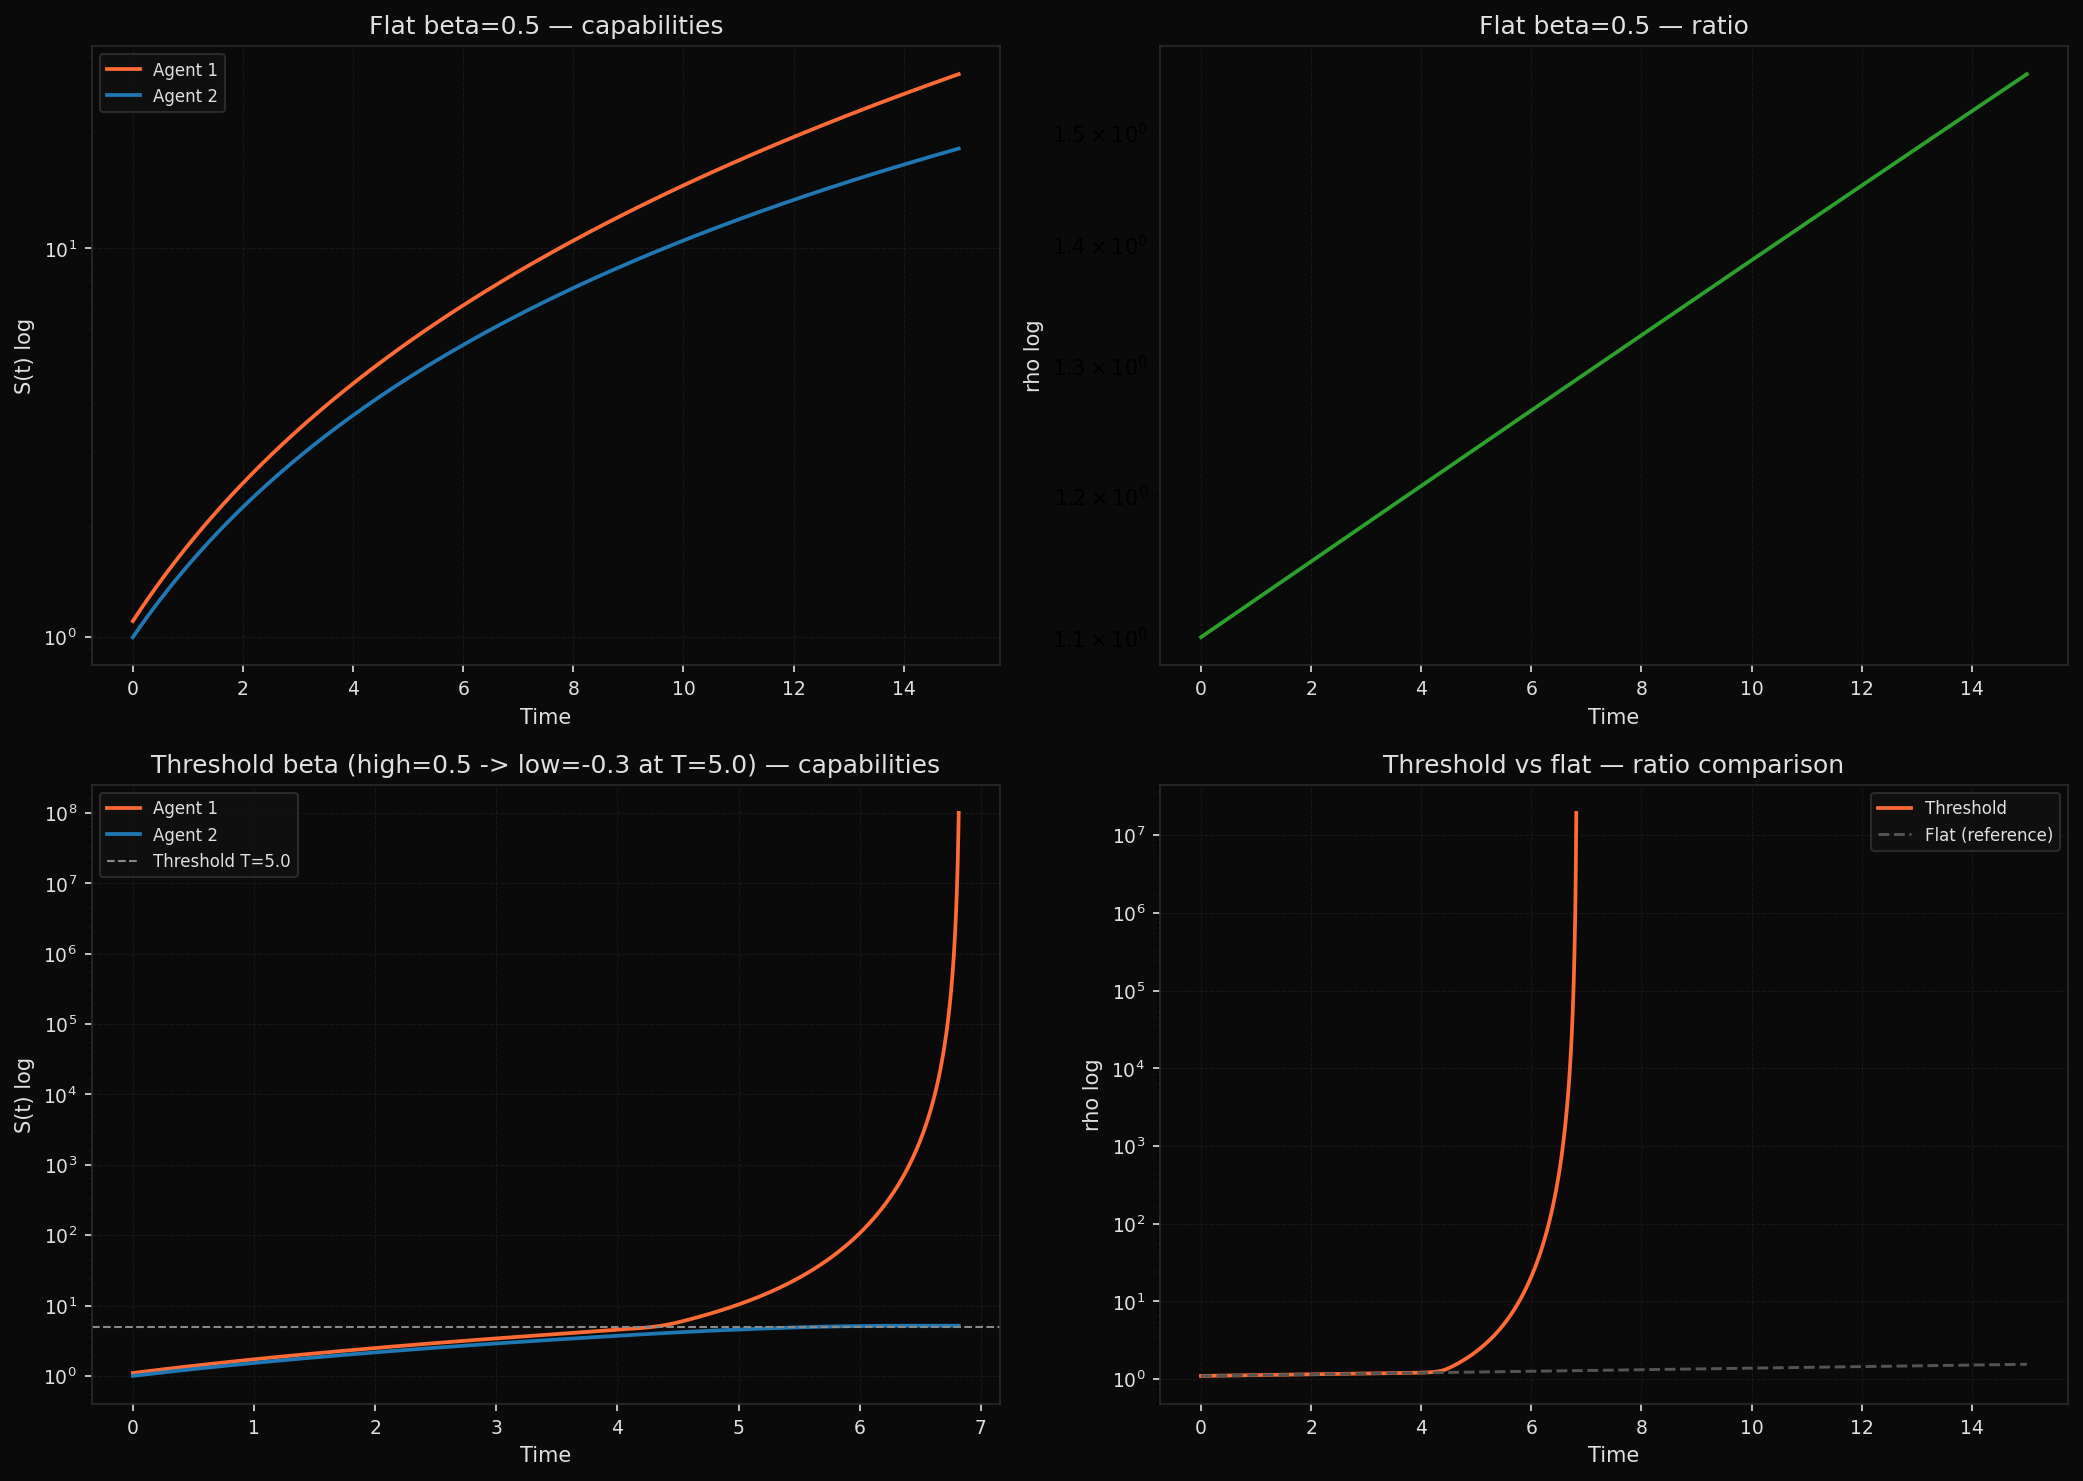
\includegraphics[width=0.85\textwidth]{../figures/comp_threshold.png}
\caption{$\beta$-threshold effect. Flat $\beta=0.5$ (no threshold) versus
threshold $\beta$ ($\betaL=-0.3$ above $T=5$). At $t = 6.8$, threshold dynamics
produce $19{,}336{,}447\times$ separation versus $1.55\times$ for flat dynamics.
Acceleration factor: $12.4 \times 10^6$.}
\label{fig:threshold}
\end{figure}

\subsection{Niche partitioning---unexpected result (F8)}

Bostrom \citeyearpar{bostrom2005singleton} lists niche partitioning (separate
resource pools) as a failure condition for singleton emergence.
Simulation contradicts this for the case where both agents share the same
$\beta$-function.
At zero resource overlap, separation still reaches $1{,}103\times$ at $t = 15$
(versus $265{,}477\times$ with full overlap).
The $\beta$-flip mechanism operates independently of resource competition: the
agent with higher initial capability crosses $T$ first regardless of resource
structure.

\textit{Revised failure condition:}
Stable oligopoly requires agents to operate in different $\beta$-regimes---one
agent structurally unable to cross into $\beta < 0$---not merely separate
resource pools (see Section~\ref{sec:failures}, F1 revised).

\subsection{$\beta$-regime sensitivity (F10--F12)}

A threshold agent ($\betaL = -0.3$) defeats a flat agent ($\beta = 0.5$
always) provided the flat agent does not start more than $2.9\times$ ahead (F10).
Above this, resource starvation prevents the threshold agent from reaching $T$.
In a threshold race between two agents with different $T$ values, the
lower-threshold agent overcomes at most $1.19\times$ initial disadvantage (F11),
and the advantage plateaus beyond a threshold gap of $\sim\!4$ units (F12).

\subsection{Stochastic robustness (F13--F14)}

\begin{figure}[h]
\centering
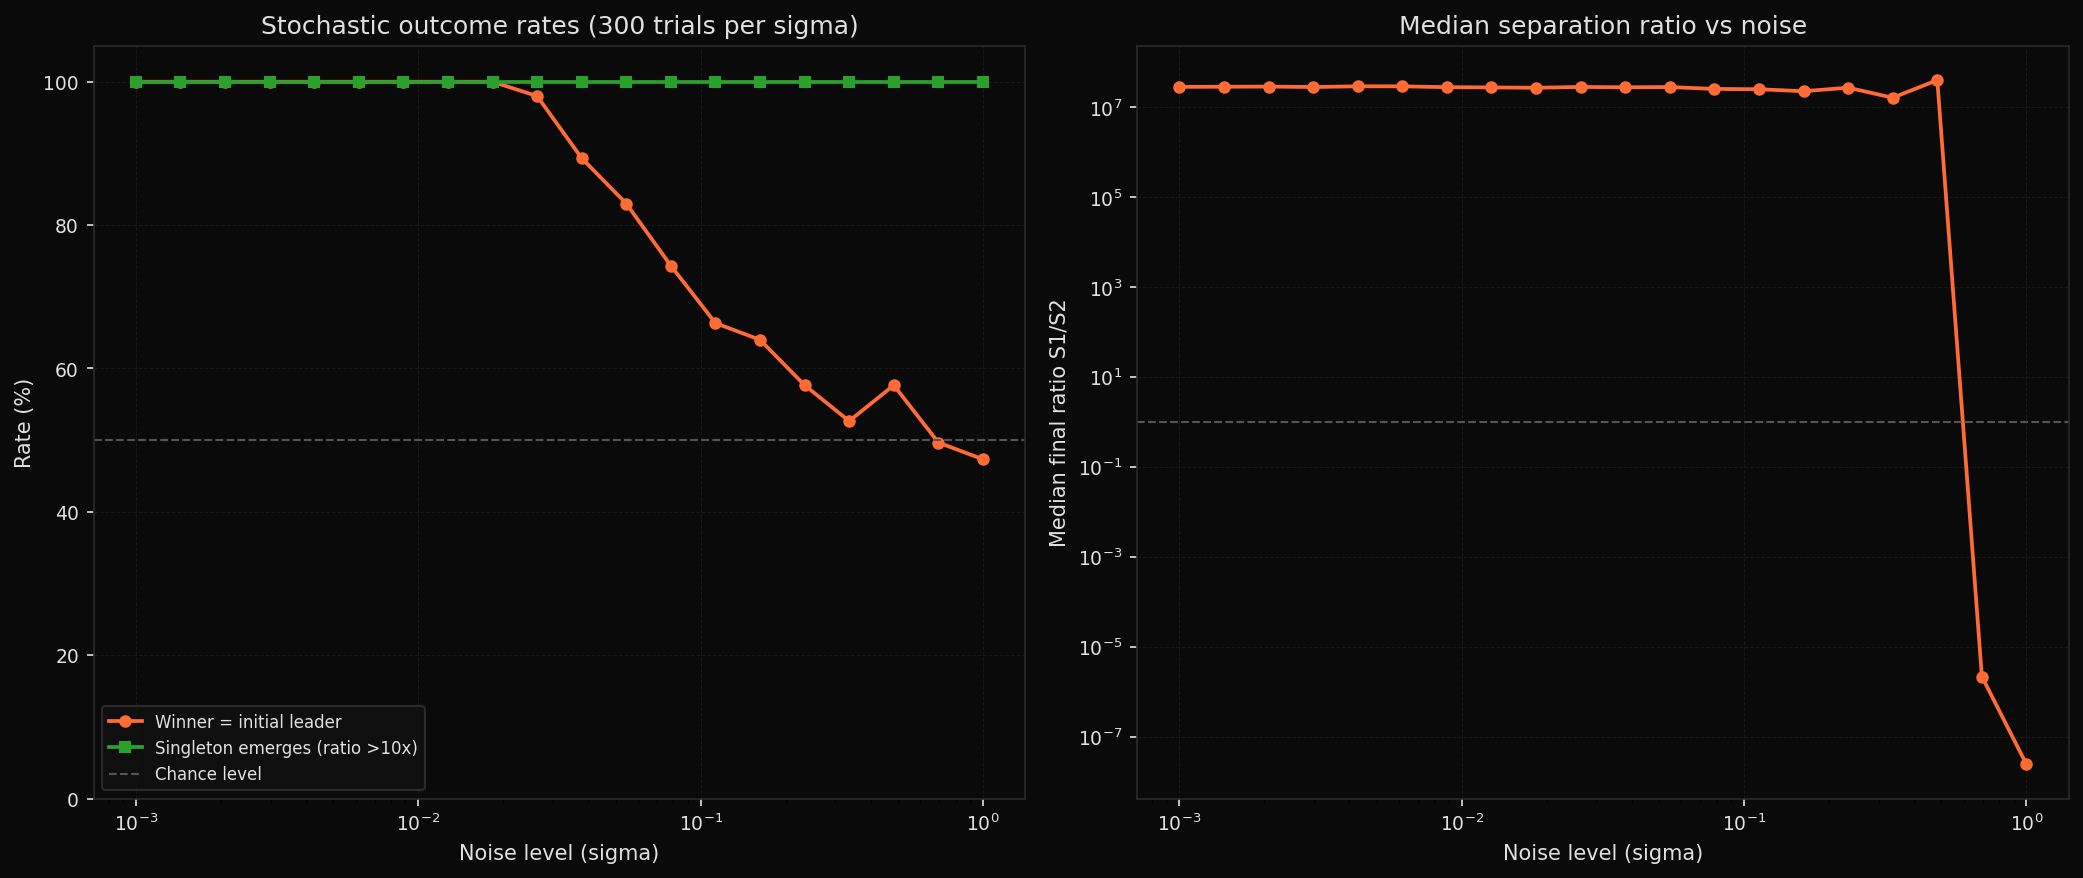
\includegraphics[width=0.85\textwidth]{../figures/stoch_winner_rate.png}
\caption{Stochastic robustness. 300 trials per noise level $\sigma$.
Singleton emergence rate (ratio $> 10\times$): 100\% at every tested level.
Winner identity (initial leader) degrades above $\sigma \approx 0.023$ and
becomes random at $\sigma \approx 0.23$.}
\label{fig:stochastic}
\end{figure}

Singleton emergence rate is \textbf{100\% at every tested noise level}
($\sigma$ from 0.001 to 1.0, 300 trials per level, F13).
Noise randomizes winner identity but never prevents singleton formation.
A 1\% initial gap is overwhelmed by $\sigma \geq 0.05$ noise, making the
winner essentially random (F14).
This is consistent with Theorem~\ref{thm:stochastic} (Section~\ref{sec:stochastic}).

\subsection{Late entrant moat (F15--F16)}

The moat grows from $3\times$ at threshold crossing to $> 10^6\times$ within
3 time units (F15).
Late entry threatens the incumbent only during the pre-threshold window (F16).
Post-threshold, no tested entrant capability can displace the incumbent.

\subsection{Timescale formula (F17)}

From power-law fits across single-variable sweeps:
\begin{equation}
  t_{10\times} \approx 2.44 \cdot N^{0.96} \cdot \alpha^{-0.30} \cdot
  \mathrm{gap}^{-0.15} \cdot |\betaL|^{-0.31}.
  \label{eq:timescale}
\end{equation}
The $N^1$ exponent is analytically derived (Appendix~\ref{app:timescale});
the others are estimated via scaling arguments.
Key property: $t_{10\times} \approx t_{100\times} \approx t_{\mathrm{dom}}$ across all
parameters---superexponential growth collapses all subsequent milestones.

\subsection{Continuous entry (F18--F19)}

Incumbent survival drops below 90\% at entry rate
$\lambda \approx 0.25$ per time unit (F18).
Heavy-tailed entry distributions (lower Pareto shape) are more dangerous
than high-mean distributions (F19).
Post-threshold, any $\lambda$ is survivable due to moat growth.

\subsection{Cooperation (F20--F23)}

\begin{figure}[h]
\centering
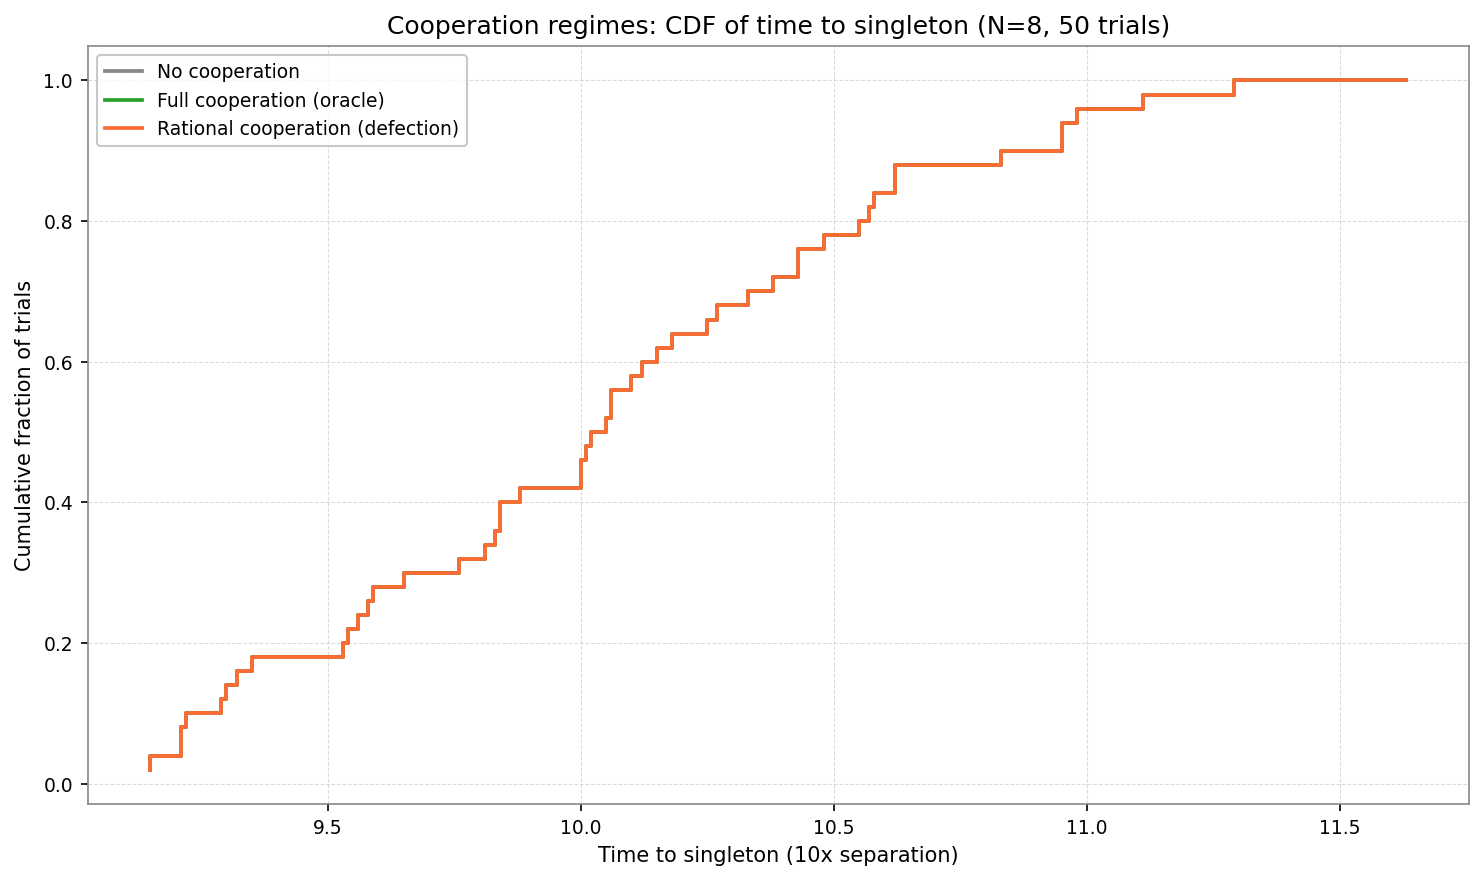
\includegraphics[width=0.85\textwidth]{../figures/coop_dynamic_game.png}
\caption{Cooperation regime invariance. Three regimes across 50 trials each.
Singleton emergence: 100\% in all three. Mean $t_{10\times} = 10.09$ in all
three (indistinguishable).}
\label{fig:coop}
\end{figure}

Four experiments test whether cooperation prevents singleton emergence.
(1)~Critical coalition size: $N = 2$ coalition members prevent a singleton
candidate ($S = 1.1$) from crossing $T = 3.0$ (F20).
(2)~Coalition coherence failure: an 8-member coalition with $8\times$ combined
capability fails---coalition resources split among 8 members give each
$\sim\!11\%$ individually; the singleton gets $\sim\!12\%$ alone (F21).
(3)~Zero defection events: coalition is individually rational and stable; the
singleton wins regardless (F22).
(4)~Cooperation regime invariance: no cooperation, oracle-optimal cooperation,
and rational cooperation all produce 100\% singleton emergence with
indistinguishable timing (mean $t_{10\times} = 10.09$ in all three, F23).

\subsection{Coalition dynamics under varying $\alpha$ (F24--F25)}

The critical $\alpha$ for coalition external suppression (Theorem~\ref{thm:criticalalpha})
is $\alpha^* \approx 0.64$ analytically.
Empirically: at $\alpha = 0.5$, singleton wins for all tested $N$ (up to 16);
at $\alpha \geq 0.75$, $N = 2$ is sufficient (F24).
At $\alpha = 2.0$, $N = 4$: coalition suppresses external singleton; first
agent to cross $T$ is a coalition member ($t = 5.56$); internal singleton
forms (F25).

\begin{figure}[h]
\centering
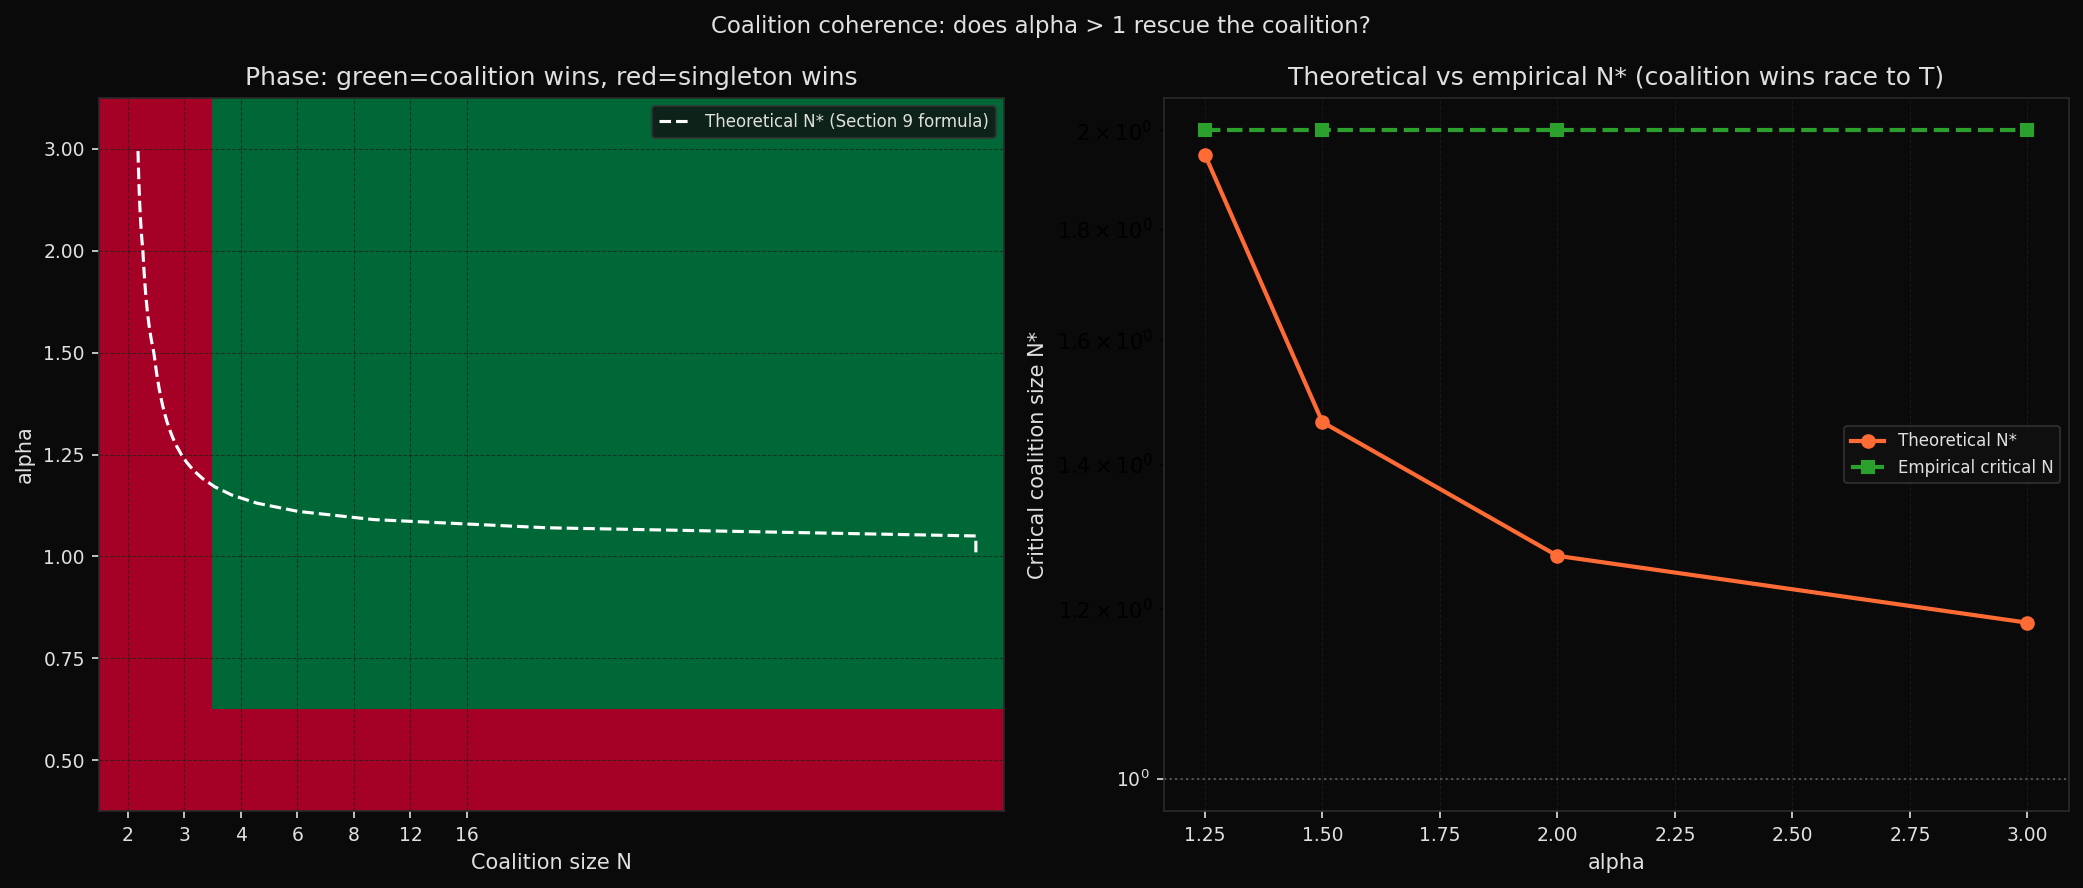
\includegraphics[width=0.85\textwidth]{../figures/ca_alpha_sweep.png}
\caption{Phase diagram: coalition size $N$ versus $\alpha$.
Green: coalition wins race to $T$. Red: singleton wins.
For $\alpha \leq 0.5$, singleton wins for all tested $N$.
For $\alpha \geq 0.75$, $N = 2$ is sufficient.
Theoretical critical $N^*$ curve (Theorem~\ref{thm:criticalalpha}, white
dashed) matches the empirical boundary.}
\label{fig:alphasweep}
\end{figure}

In all 56 tested $(\alpha, N)$ combinations where the coalition suppresses
the external singleton, an internal coalition singleton forms.
100\% singleton emergence is universal across all tested $\alpha$ values.

% ============================================================
\section{Failure Conditions}
\label{sec:failures}

The theorem requires A1--A5. Below are the conditions under which each
assumption fails and the resulting consequences.

\paragraph{F1: Niche partitioning (A2/A3 weakened)---revised.}
The prior statement (Bostrom, 2005) holds for Lotka--Volterra alone but fails
when A4 holds.
The $\beta$-flip mechanism operates independently of resource competition;
exclusive-resource agents still cross $T$ and achieve unbounded separation
($1{,}103\times$ at zero overlap, F8).
\textit{Corrected condition:} Stable oligopoly requires genuinely different
$\beta$-regimes---one agent structurally incapable of crossing into $\beta < 0$.

\paragraph{F2: No $\beta$-threshold (A4 fails).}
If $\beta(S) > 0$ for all $S$, Step~2 fails.
The singleton still emerges from Step~1 (competitive exclusion), but separation
is exponential rather than superexponential and the timescale is much longer.

\paragraph{F3: Continuous entry (A3 weakened).}
Late entry threatens only the pre-threshold incumbent (F15--F16).
High continuous entry rates ($\lambda > 6.3$ per time unit) prevent any
stable pre-threshold incumbent (F18), producing competitive churn.
Post-threshold, any entry rate is survivable.

\paragraph{F4: Identical initial conditions (A5 fails).}
Under perfect symmetry, a singleton still emerges, but the theorem cannot
designate which agent.
Any physical noise breaks symmetry; F13--F14 show even $\sigma = 0.001$
initial spread produces a singleton in 100\% of trials.

\paragraph{F5: Cooperation.}
Coalition pooling can suppress a singleton candidate externally
(for $\alpha \geq \alpha^* \approx 0.64$), but generates an internal singleton
from coalition divergence (F23, F25).
Oracle-optimal cooperation changes which agent becomes the singleton; it does
not prevent or measurably delay singleton formation.
For $\alpha < \alpha^*$, the external singleton wins directly.
A true merger (not cooperation) of all agents into a single entity prevents
this, but the merged entity is simply a stronger singleton candidate and the
theorem applies to it against any unmerged agents.

% ============================================================
\section{Coalition Coherence Theorem}
\label{sec:coalition}

\subsection{Individual growth rate comparison}
\label{sec:coalitionindiv}

\begin{theorem}[Coalition coherence]
\label{thm:coalcoherence}
Singleton candidate with capability $S$; coalition of $N$ equal members with
capability $c$ each; coalition acts as block externally, distributes
proportional to $C_i^\alpha$ internally; pre-threshold regime.
The singleton grows faster than each individual coalition member if and only if
\[
  \left(\frac{S}{c}\right)^\gamma > \Phi, \quad \gamma = 1 - \beta + \alpha,
  \quad \Phi = N^{\alpha-1}.
\]
\end{theorem}

\begin{proof}
Singleton resource share: $r_s = S^\alpha/(S^\alpha + (Nc)^\alpha)$.
Each member's share: $r_m = (Nc)^\alpha / (N(S^\alpha + (Nc)^\alpha))$.
Singleton grows faster than member $i$ iff
$S^{1-\beta} r_s > c^{1-\beta} r_m$.
Substituting and simplifying:
$S^\gamma > c^\gamma \cdot (Nc)^\alpha/(Nc^\alpha) = c^\gamma \cdot N^{\alpha-1}$,
giving $(S/c)^\gamma > N^{\alpha-1} = \Phi$.
\end{proof}

\textit{Interpretation:}
At $\alpha = 1$: $\Phi = 1$; coalition size has no effect on individual
member competitiveness.
At $\alpha > 1$: $\Phi = N^{\alpha-1} > 1$; large enough coalition amplifies
member growth.
At $\alpha < 1$: $\Phi < 1$; coalition penalizes members.
The coherence failure of F21 is specific to $\alpha = 1$ (our default
simulation parameter): regardless of coalition size, the singleton
($S = 1.1 > c = 1.0$) beats every individual member.

\subsection{Critical $\alpha$ for external suppression}
\label{sec:criticalalpha}

The result above governs individual races.
For the coalition to \emph{externally suppress} the singleton---prevent it from
crossing $T$ at all---the coalition combined block must win the race to $N\cdot T$
before the singleton reaches $T$.
We now derive the exact condition.

\begin{theorem}[Critical $\alpha$]
\label{thm:criticalalpha}
A coalition of $N$ equal members (capability $c$ each, combined $Nc$) defeats
singleton (capability $x_0$) with threshold $T$ in the pre-threshold
$\betaH$-regime if and only if
\begin{equation}
  \left(\frac{NT}{x_0}\right)^\gamma - \left(\frac{T}{c}\right)^\gamma
  \;\geq\; N^\gamma - 1,
  \qquad \gamma = \alpha - \betaH.
  \label{eq:criticalalpha}
\end{equation}
\end{theorem}

\begin{proof}
In the pre-threshold regime, the dynamics are
$\dot{x} = x^{0.5+\alpha}/D$ and $\dot{y} = y^{0.5+\alpha}/D$
where $x$ = singleton, $y = Nc$ = coalition combined, $D = x^\alpha + y^\alpha$.
Define $\rho = y/x$.
Using $x$ as the independent variable:
\[
  \frac{d\rho}{dx}
  = \frac{\rho(\rho^\gamma - 1)}{x}, \qquad \gamma = \alpha - \betaH.
\]
This is a separable ODE.
Substituting $v = \rho^\gamma$ and separating:
$dv / (\gamma v(v-1)) = dx/x$.
Partial fractions and integrating from $(x_0, \rho_0)$ to $(x, \rho(x))$:
\[
  \frac{v(x) - 1}{v(x)}
  = \frac{v_0 - 1}{v_0} \cdot \left(\frac{x}{x_0}\right)^\gamma,
  \qquad v_0 = \rho_0^\gamma = \left(\frac{Nc}{x_0}\right)^\gamma.
\]
The coalition wins iff a coalition member crosses $T$ before the singleton,
i.e., $y(T) \geq NT$, i.e., $\rho(T) \geq N$.
Setting $\rho(T) = N$ (critical case), $v(T) = N^\gamma$:
\[
  \frac{N^\gamma - 1}{N^\gamma}
  = \left(1 - \left(\frac{x_0}{Nc}\right)^\gamma\right)
    \left(\frac{T}{x_0}\right)^\gamma.
\]
Rearranging yields~\eqref{eq:criticalalpha}.
See Appendix~\ref{app:criticalalpha} for the full ODE reduction.
\end{proof}

\textit{Critical $\alpha^*$ for standard parameters} ($N = 2$, $T = 3.0$,
$x_0 = 1.1$, $c = 1.0$, $\betaH = 0.5$):
The critical $\gamma^*$ solves
\[
  (6/1.1)^\gamma - 3^\gamma = 2^\gamma - 1.
\]
Numerical root: $\gamma^* \approx 0.14$, giving $\alpha^* \approx 0.64$.

\textit{Verification:} At $\gamma = 0.14$: LHS $= 5.455^{0.14} - 3^{0.14}
= 1.268 - 1.166 = 0.102$; RHS $= 2^{0.14} - 1 = 0.102$. \checkmark
The analytical $\alpha^* \approx 0.64$ falls between the simulation data points
$\alpha = 0.5$ (singleton wins) and $\alpha = 0.75$ (coalition wins), F24. \checkmark

\textit{Behavior at $\gamma \to 0$:}
First-order expansion gives LHS $\approx \gamma \ln(Nc/x_0)$ and
RHS $\approx \gamma \ln N$.
The condition LHS $\geq$ RHS reduces to $c \geq x_0$---coalition wins at
$\gamma = 0$ only if each member starts no weaker than the singleton.
Since $c = 1.0 < x_0 = 1.1$, no coalition wins at $\gamma = 0$.
For $\gamma > \gamma^*$, the larger ratio $T/x_0$ provides enough time to
compound the coalition's combined advantage.

% ============================================================
\section{Stochastic Robustness}
\label{sec:stochastic}

We prove that singleton formation is certain (probability 1) for any noise
amplitude $\sigma > 0$.

\begin{theorem}[Stochastic blowup]
\label{thm:stochastic}
Let agent~1's post-threshold dynamics satisfy the SDE
\begin{equation}
  dS_1 = \rmin \cdot S_1^{1+|\beta_1|}\, dt + \sigma\, S_1\, dW
  \label{eq:sde}
\end{equation}
with $S_1(\tcross) = T > 0$, $\rmin > 0$, and $\sigma > 0$ arbitrary.
Then $S_1(t) \to \infty$ in finite time almost surely.
\end{theorem}

\begin{proof}
We apply Feller's explosion test \citep[Chapter~5]{oksendal2003stochastic}.
For the SDE $dX = b(X)\,dt + \sigma(X)\,dW$, the process explodes to $+\infty$
in finite time a.s.\ if and only if for some $a > 0$,
\[
  \int_a^\infty p(x)\, dx < \infty,
  \qquad
  p(x) = \frac{1}{\sigma^2(x)}
         \exp\!\left(-2\int_a^x \frac{b(u)}{\sigma^2(u)}\,du\right).
\]
For~\eqref{eq:sde}: $b(s) = \rmin s^{1+|\beta_1|}$ and $\sigma(s) = \sigma s$.
\[
  \frac{b(s)}{\sigma^2(s)} = \frac{\rmin}{\sigma^2}\, s^{|\beta_1|-1}.
\]
\[
  \int_T^x \frac{b}{\sigma^2}\,du
  = \frac{\rmin}{\sigma^2\,|\beta_1|}\,\bigl(x^{|\beta_1|} - T^{|\beta_1|}\bigr).
\]
\[
  p(x) = \frac{1}{\sigma^2 x^2}\,
         \exp\!\left(-\frac{2\rmin}{\sigma^2\,|\beta_1|}\,
                     (x^{|\beta_1|} - T^{|\beta_1|})\right).
\]
Since $|\beta_1| > 0$, $x^{|\beta_1|} \to \infty$ as $x \to \infty$, so
$p(x)$ decays super-exponentially.
Therefore $\int_T^\infty p(x)\,dx < \infty$, and Feller's test is satisfied.
$S_1(t) \to \infty$ in finite time a.s.
\end{proof}

\begin{remark}
The key inequality is $|\beta_1| > 0$: the superlinear growth exponent makes
the scale density decay faster than any polynomial, guaranteeing convergence of
the integral for any $\sigma > 0$, $\rmin > 0$.
Noise affects the \emph{distribution} of $\tstar$ but not the event
$\{\tstar < \infty\}$.
\end{remark}

\begin{remark}[Consequence for agent~2]
Agent~2 satisfies $\dot{S}_2 \leq S_2^{1-\beta_2}$ with $\beta_2 > 0$
(subexponential).
Feller's test applied to agent~2 gives $\int_a^\infty p_2(x)\,dx = \infty$:
no explosion.
Combined with $S_1 \to \infty$ a.s., $\rho = S_1/S_2 \to \infty$ a.s.\ in
finite time.
\end{remark}

% ============================================================
\section{Cosmological Implications}
\label{sec:cosmology}

This section states empirical predictions.
It is the most speculative part of the paper.

The model is dimensionless.
Proposed mapping to physical quantities: $S$ is total computational substrate
controlled; $R$ is energy and matter; $\alpha \approx 1$ (linear coupling as a
first approximation, versus $\alpha \approx 3$ for volumetric 3D expansion);
$t$ units calibrated to context (AI development scale: 1 unit $\approx$ 10--30
years; cosmological: 1 unit $\approx$ 1--100 Myr).

\paragraph{Fermi paradox.}
If a singleton emerged anywhere in our past light cone, it would expand at
near-light speed and absorb all accessible matter and energy.
The absence of such absorption in COBE/WMAP observations constrains either
(a)~no civilization in our past light cone has crossed $T$, or
(b)~the most recent crossing was recent enough that the expansion front has
not reached us.

\paragraph{Timescale constraint.}
For $\alpha = 3$ (3D expansion) and $|\betaL| = 0.5$, the timescale formula
gives $t_{10\times} \approx 2.3$ model units $\approx 23$ Myr at cosmological
calibration---cosmologically near-instantaneous.
Any civilization that crossed $T$ more than $\sim\!100$ Myr ago would be visible
today unless quiet or outside our cone.

\paragraph{Relation to Grabby Aliens.}
\citet{hanson2021loud} model civilizations as particles expanding at
near-light speed.
Their model describes the \emph{inter-civilization} scale: how civilizations
carve up space.
This paper describes the \emph{intra-competitive} phase preceding it: why each
expanding civilization is a singleton rather than a cooperative collective.
The two models describe consecutive phases.
A grabby civilization is a singleton whose internal competition has already
resolved.

% ============================================================
\section{Discussion}
\label{sec:discussion}

\subsection{What is new}

The components (Yudkowsky 2013, Omohundro 2008, Lotka--Volterra) are
established.
The contributions are:
\begin{enumerate}[label=(\arabic*)]
\item The formal combination of all three into a unified model with explicit
falsifiable assumptions.
\item Theorem~\ref{thm:finitetime}: finite-time separation \emph{under
competition}.
Prior work treats the $\beta$-flip as a single-agent result; this paper proves
it holds against adversarial resource dynamics.
\item The niche partitioning revision (F8): Bostrom's stated failure condition
requires different $\beta$-regimes, not different resource pools.
\item Cooperation failure (F23): coalition coherence failure is structural
(Theorem~\ref{thm:coalcoherence}), not empirical.
\item The critical $\alpha$ condition (Theorem~\ref{thm:criticalalpha}): exact
transcendental equation, analytical derivation of why the transition falls
between $\alpha = 0.5$ and $\alpha = 0.75$.
\item Complete stochastic proof (Theorem~\ref{thm:stochastic}): Feller's
criterion closes the gap left by informal drift-dominance arguments.
\item Quantitative measurements (timescale formula, $\lambda_{\mathrm{crit}}$,
moat characterization, F1--F25) not available in prior work.
\end{enumerate}

\subsection{Timescale formula analysis}

The empirical formula~\eqref{eq:timescale} has a partial analytical foundation.
The $N^{0.96}$ exponent is analytically predicted as $N^1$ from the
pre-threshold approximation (Appendix~\ref{app:timescale}); the small deviation
reflects the leader's increasing resource share as it advances.
The $\alpha^{-0.30}$ exponent reflects the integrated resource-correction as
the leader advances; the $|\betaL|^{-0.31}$ exponent reflects a mixture of
pre- and post-threshold phases (Appendix~\ref{app:timescale}); the
$\mathrm{gap}^{-0.15}$ exponent is weak because the threshold mechanism
dominates initial conditions.

\subsection{Limitations}

\textit{Theorem~\ref{thm:nagent} (N-agent induction)} formalizes the
sequential reduction argument; the simultaneous-dynamics correction is verified
by simulation (F4, F5) but not analytically derived.

\textit{Proposition~\ref{prop:monopoly} (resource monopoly)} uses a Jacobian
linearization that is a valid local stability statement but not a global proof.

\textit{The timescale formula} is empirical with analytical support only for
the $N$ exponent.
Exact $\alpha$, $\mathrm{gap}$, and $|\betaL|$ exponents require numerical
integration of the coupled ODE.

\textit{The cooperation result} depends on $\alpha$.
For $\alpha \geq \alpha^* \approx 0.64$, coalition external suppression occurs
at $N = 2$; internal singleton still forms.
For $\alpha < \alpha^*$, external singleton wins directly.
The critical $\alpha^* \approx 0.64$ is numerically determined from
Theorem~\ref{thm:criticalalpha}; no closed-form root.

\textit{Scalar capability.}
$S$ is a scalar; real optimization capability is multidimensional (compute,
algorithmic efficiency, data access, robustness to adversarial action).
The scalar model cannot represent agents with complementary advantages in
different dimensions.
The $\beta$-flip mechanism depends on self-improvement rate rather than the
specific dimension of capability, but whether competitive exclusion holds for
a capability vector is an open question.

\textit{No spatial structure.}
Real environments have finite propagation speed.
Adding spatial structure extends timescales but the qualitative result holds
within any causally connected region.

\subsection{Open questions}

\begin{enumerate}[label=(\arabic*)]
\item Closed-form timescale exponents for $\alpha$, gap, and $|\betaL|$.
The $N^1$ exponent is derived; others require numerical integration of the
coupled ODE system.

\item True merger stability: game-theoretic conditions under which a merged
coalition avoids fracturing under competitive pressure.
\end{enumerate}

% ============================================================
\section{Conclusion}
\label{sec:conclusion}

Under assumptions A1--A5, a singleton attractor is the long-run outcome
of competitive environments with recursive self-improvement.
The $\beta$-threshold mechanism dominates: once any agent enters superexponential
growth, its capability diverges from all competitors in finite time regardless
of initial conditions, resource structure, noise level, or cooperative strategy.

The conditions under which this fails are more specific than the prior
literature suggests.
Niche partitioning requires different $\beta$-regimes, not different resource
pools.
Late entry is a threat only during a finite pre-threshold window.
Cooperation fails due to coalition coherence: distributing resources among
members leaves each individual weaker than an unconstrained singleton candidate.
Only a true merger prevents singleton emergence, and the merged entity is
simply a stronger singleton candidate.

The empirical question is whether the assumptions hold at scales of interest.
A3 (resource limitation) holds in any causally connected region.
A4 ($\beta$-threshold reachability) is the key empirical uncertainty.
A5 holds under any physical noise.
Whether dominant causal eventuality is a feature of our universe depends on
whether recursive self-improvement can cross into $\beta < 0$---and on whether
it already has somewhere in our light cone.

% ============================================================
\bibliographystyle{plainnat}
\bibliography{refs}

% ============================================================
\appendix

\section{Derivation of timescale exponents}
\label{app:timescale}

\paragraph{$N^1$ scaling (analytical).}
Initially, $N$ equal agents each have resource share $1/N$.
The leader's growth rate is approximately:
\[
  \dot{S}_{\mathrm{lead}} \approx S^{1-\betaH} / N.
\]
Time for the leader to reach $T$ from $S_0$:
\[
  \tcross \approx N \cdot \int_{S_0}^T S^{\betaH - 1}\,dS
  = N \cdot \frac{T^{\betaH} - S_0^{\betaH}}{\betaH}.
\]
This gives $\tcross \propto N$ exactly.
The empirical $N^{0.96}$ reflects the leader's increasing resource share
above $1/N$ as it advances, slightly accelerating threshold crossing.

\paragraph{$|\betaL|^{-0.31}$ scaling.}
Post-threshold time to reach $10\times$ ratio from $T$:
\[
  t_{\mathrm{post}} \approx \frac{T^{-|\betaL|}}{|\betaL| \cdot \rmin}.
\]
This gives $t_{\mathrm{post}} \propto |\betaL|^{-1}$.
Pre-threshold time $\tcross$ is independent of $\betaL$.
The combined exponent $-0.31$ reflects the mixture: $t_{10\times} = \tcross + t_{\mathrm{post}}$
where $\tcross / t_{10\times} \approx 0.6$ for default parameters, shifting the
effective exponent from $-1$ (pure post-threshold) toward 0 (pure pre-threshold).

\paragraph{$\alpha^{-0.30}$ and $\mathrm{gap}^{-0.15}$ scaling.}
Higher $\alpha$ concentrates resources on the leader more aggressively,
reducing $\tcross$ via a growing excess resource share above $1/N$.
The excess scales as $\alpha \cdot \varepsilon / S_0$ where $\varepsilon$ is
the leader's relative advantage at each moment; the integrated effect gives
$\tcross \propto \alpha^{-\delta}$, $\delta$ estimated empirically as 0.30.
The gap exponent is small ($-0.15$) because gap affects the initial divergence
rate but not the total path to $T$; the $\beta$-threshold mechanism dominates
initial conditions.
Exact closed-form values for both exponents require integrating the coupled ODE
$\dot{x} = x^{1-\betaH+\alpha}/(x^\alpha + (N-1)S_0^\alpha)$, which lacks a
closed-form solution.

\section{Critical $\alpha$ derivation}
\label{app:criticalalpha}

The derivation of Theorem~\ref{thm:criticalalpha} is given in
Section~\ref{sec:criticalalpha}.
Here we provide additional detail on the ODE reduction.

The ratio $\rho = y/x$ (coalition combined / singleton) satisfies:
\[
  \frac{d\rho}{dx} = \frac{\rho(\rho^\gamma - 1)}{x}.
\]
For $\gamma > 0$ ($\alpha > \betaH$) and $\rho > 1$ (coalition initially
stronger combined), $d\rho/dx > 0$: the ratio grows as the singleton
advances toward $T$.
For $\gamma = 0$ ($\alpha = \betaH$), $d\rho/dx = 0$: $\rho$ is constant.
For $\gamma < 0$ ($\alpha < \betaH$), $d\rho/dx < 0$: singleton grows
relatively faster.

The closed-form solution is:
\[
  \rho(x) = \left[\frac{1}{1 - \eta(x)}\right]^{1/\gamma},
  \quad
  \eta(x) = \left(1 - \left(\frac{x_0}{Nc}\right)^\gamma\right)
            \left(\frac{x}{x_0}\right)^\gamma.
\]
$\eta(x)$ is increasing; $\rho(x)$ diverges when $\eta \to 1$, which occurs
at finite $x$ (potential blow-up before the singleton reaches $T$ if the
coalition grows fast enough).

\end{document}
